\chapter{Artificial Intelligence (AI) \cite{aci-1}}

\begin{enumerate}[itemsep=0.2cm]
    \item The field of artificial intelligence, or AI, attempts not just to understand but also to build intelligent entities. 

    \item \textbf{Acting humanly}: \textit{Turing test}
    \begin{enumerate}
        \item The \textbf{Turing Test}\indexlabel{Turing Test}, proposed by Alan Turing (1950), was designed to provide a satisfactory operational definition of intelligence.\\
        A computer passes the test if a human interrogator, after posing some written questions, cannot tell whether the written responses come from a person or from a computer.\\
        total Turing Test includes a video signal so that the interrogator can test the subject’s perceptual abilities, as well as the opportunity for the interrogator to pass physical objects “through the hatch.”\\
        To pass the total Turing Test, the computer will need:
        \begin{enumerate}
            \item \textbf{computer vision} to perceive objects

            \item \textbf{robotics} to manipulate objects and move about
        \end{enumerate}

        \item The computer would need to possess the following capabilities: 
        \begin{enumerate}
            \item \textbf{natural language processing} to enable it to communicate successfully in English

            \item \textbf{knowledge representation} to store what it knows or hears

            \item \textbf{automated reasoning} to use the stored information to answer questions and to draw new conclusions

            \item \textbf{machine learning} to adapt to new circumstances and to detect and extrapolate patterns
        \end{enumerate}
    \end{enumerate}

    \item \textbf{Thinking humanly}: \textit{The cognitive modeling approach} 
    \begin{enumerate}
        \item The interdisciplinary field of \textbf{cognitive science}\indexlabel{cognitive science} brings together computer models from AI and experimental techniques from psychology to construct precise and testable theories of the human mind. 

        \item an algorithm performs well on a task and that it is therefore a good model of human performance, or vice versa.
    \end{enumerate}

    \item \textbf{Thinking rationally}: \textit{The “laws of thought” approach}
    \begin{enumerate}
        \item The Greek philosopher Aristotle was one of the first to attempt to codify “right thinking,” that is, irrefutable reasoning processes

        \item His syllogisms/ arguments provided patterns for argument structures that always yielded correct conclusions when given correct premises-for example, \textit{“Socrates is a man; all men are mortal; therefore, Socrates is mortal.”}

        \item logicist tradition within artificial intelligence hopes to build on such programs to create intelligent systems. \\
        There are two main obstacles to this approach.
        \begin{enumerate}
            \item it is not easy to take informal knowledge and state it in the formal terms required by logical notation, particularly when the knowledge is less than 100\% certain

            \item there is a big difference between solving a problem “in principle” and solving it in practice.
        \end{enumerate}
    \end{enumerate}

    \item \textbf{Acting rationally}: \textit{The rational agent approach}
    \begin{enumerate}
        \item An \textbf{agent}\indexlabel{agent} is just something that acts (agent comes from the Latin agere, to do).\\
        Of course, all computer programs do something, but computer agents are expected to do more: operate autonomously, perceive their environment, persist over a prolonged time period, adapt to change, and create and pursue goals. 
        
        \item A \textbf{rational agent}\indexlabel{rational agent} is one that acts so as to achieve the best outcome or, when there is uncertainty, the best expected outcome.

        \item In the \textit{“laws of thought” approach} to AI, the emphasis was on correct inferences.\\
        Making correct inferences is sometimes part of being a rational agent, because one way to act rationally is to reason logically to the conclusion that a given action will achieve one’s goals and then to act on that conclusion.\\
        On the other hand, correct inference is not all of ration-ality; in some situations, there is no provably correct thing to do, but something must still be done.\\
        There are also ways of acting rationally that cannot be said to involve inference.\\
        \textbf{For example}, recoiling from a hot stove is a reflex action that is usually more successful than a slower action taken after careful deliberation.

        \item The rational-agent approach has two advantages over the other approaches. 
        \begin{enumerate}
            \item it is more general than the “laws of thought” approach because correct inference is just one of several possible mechanisms for achieving rationality. 

            \item it is more amenable to scientific development than are approaches based on human behavior or human thought. 
        \end{enumerate}

        \item The standard of rationality is mathematically well defined and completely general, and can be “unpacked” to generate agent designs that provably achieve it.\\
        Human behavior, on the other hand, is well adapted for one specific environment and is defined by, well, the sum total of all the things that humans do.

        \item \textbf{limited rationality}\indexlabel{limited rationality} - acting appropriately when there is not enough time to do all the computations one might like.
    \end{enumerate}
\end{enumerate}

\section{Fundamentals of AI \cite{aci-1}}

\subsection{Philosophy}
\begin{enumerate}
    \item \textbf{rationalism}\indexlabel{rationalism} Descartes was a strong advocate of the power of reasoning in understanding the world, a philosophy now called rationalism, and one that counts Aristotle and Leibnitz as members. 

    \item \textbf{dualism}\indexlabel{dualism}: Descartes was also a proponent of dualism.\\
    He held that there is a part of the human mind (or soul or spirit) that is outside of nature, exempt from physical laws.\\
    Animals, on the other hand, did not possess this dual quality; they could be treated as machines.

    \item \textbf{materialism}\indexlabel{materialism}: An alternative to dualism is materialism, which holds that the brain’s operation according to the laws of physics constitutes the mind.\\
    Free will is simply the way that the perception of available choices appears to the choosing entity.

    \item \textbf{empiricism}\indexlabel{empiricism}: the theory that all knowledge is based on experience derived from the senses.

    \item \textbf{induction}\indexlabel{induction}: that general rules are acquired by exposure to repeated associations between their elements.

    \item \textbf{logical positivism}\indexlabel{logical positivism}: holds that all knowledge can be characterized by logical theories connected

    \item \textbf{confirmation theory}\indexlabel{confirmation theory}: to analyze the acquisition of knowledge from experience

    \item the mind is the connection between knowledge and action

    \item because intelligence requires action as well as reasoning

    \item only by understanding how actions are justified can we understand how to build an agent whose actions are justifiable (or rational)
\end{enumerate}

\subsection{Mathematics}
\begin{enumerate}
    \item leap to a formal science required a level of mathematical formalization in three fundamental areas: logic, computation, and probability.

    \subsubsection*{Logic}

    \item The idea of formal logic can be traced back to the philosophers of \textbf{ancient Greece} who worked out the details of propositional, or Boolean logic.

    \item In 1879, \textbf{Gottlob Frege} (1848–1925) extended Boole’s logic to include objects and relations, creating the \textit{first-order logic}\\
    first-order logic could \textbf{not} capture the principle of mathematical induction needed to characterize the natural numbers.

    \item \textbf{Alfred Tarski} (1902–1983) introduced a theory of reference that shows how to relate the objects in a logic to objects in the real world.

    \item \textbf{algorithm}: a process or set of rules to be followed in calculations or other problem-solving operations, especially by a computer.\\
    The first nontrivial algorithm is thought to be Euclid’s algorithm for computing greatest common divisors.

    \item In 1931, Godel showed that limits on deduction do exist.\\
    His \textbf{incompleteness theorem}\indexlabel{incompleteness theorem} showed that in any formal theory as strong as Peano arithmetic (the elementary theory of natural numbers), there are true statements that are undecidable in the sense that they have no proof within the theory. \\
    some functions on the integers cannot be represented by an algorithm - that is, they cannot be computed. \\
    the notion of a computation or effective procedure really cannot be given a formal definition

    \subsubsection*{Computation}

    \item \textbf{Church–Turing thesis}\indexlabel{Church–Turing thesis}, which states that the Turing machine (Turing, 1936) is capable of computing any computable function, is generally accepted as providing a sufficient definition.\\
    Turing also showed that there were some functions that no Turing machine can compute.\\
    \textbf{For example}, no machine can tell in general whether a given program will return an answer on a given input or run forever. 

    \item a problem is called \textbf{intractable} if the time required to solve instances of the problem grows exponentially with the size of the instances.\\
    It is important because exponential growth means that even moderately large instances cannot be solved in any reasonable time.\\
    Therefore, one should strive to divide the overall problem of generating intelligent behavior into tractable subproblems rather than intractable ones. 

    \item theory of \textbf{NP-completeness}: \textbf{Steven Cook} (1971) and \textbf{Richard Karp} (1972) showed the existence of large classes of canonical combinatorial search and reasoning problems that are NP-complete.\\
    Any problem class to which the class of NP-complete problems can be reduced is likely to be intractable. (Although it has not been proved that NP-complete problems are necessarily intractable)

    \subsubsection*{Probability}

    \item Italian \textbf{Gerolamo Cardano} (1501–1576) first framed the idea of \textbf{probability}, describing it in terms of the possible outcomes of gambling events.
\end{enumerate}

\subsection{Economics}
\begin{enumerate}
    \item Most people think of economics as being about money, but economists will say that they are really studying how people make choices that lead to preferred outcomes. 

    \item \textbf{utility}: useful, profitable, or beneficial\\
    The mathematical treatment of “preferred outcomes” or utility was first formalized by \textbf{Leon Walras} (1834-1910)

    \item \textbf{Decision theory}, which combines probability theory with utility theory, provides a formal and complete framework for decisions (economic or otherwise) made under uncertainty - that is, in cases where probabilistic descriptions appropriately capture the decision maker’s environment.\\
    This is suitable for \textit{“large” economies} where each agent need pay no attention to the actions of other agents as individuals.

    \item For \textit{“small” economies}, the situation is much more like a \textbf{game}: the actions of one player can significantly affect the utility of another (either positively or negatively).\\
    \textbf{Von Neumann} and \textbf{Morgenstern}’s development of \textbf{game theory} included the surprising result that, for some games, a rational agent should adopt policies that are (or least appear to be) randomized.\\
    Unlike decision theory, game theory does not offer an unambiguous prescription for selecting actions.

    \item The topic of \textit{"ow to make rational decisions when payoffs from actions are not immediate but instead result from several actions taken in sequence"} was pursued in the field of \textbf{operations research}, which emerged in World War II from efforts in Britain to optimize radar installations.\\
    The work of Richard Bellman (1957) formalized a class of sequential decision problems called \textbf{Markov decision processes} (MDP).

    \item models based on satisficing - making decisions that are “good enough,” rather than laboriously calculating an optimal decision - gave a better description of actual human behavior.
\end{enumerate}

\subsection{Neuroscience}
\begin{enumerate}
    \item Neuroscience is the study of the nervous system, particularly the brain.

    \item brain consisted of nerve cells, or neurons

    \item computers have a cycle time that is a million times faster than a brain.\\
    The brain makes up for that with far more storage and interconnection than even a high-end personal computer, although the largest supercomputers have a capacity that is similar to the brain’s.
\end{enumerate}

\subsection{Psychology}
\begin{enumerate}
    \item \textbf{Behaviorism movement}, led by \textbf{John Watson} (1878–1958), rejected any theory involving mental processes on the grounds that introspection could not provide reliable evidence. \\
    Behaviorists insisted on studying only objective measures of the percepts (or stimulus) given to an animal and its resulting actions (or response). 

    \item \textbf{Cognitive psychology} views the brain as an information-processing device.

    \item Helmholtz also insisted that perception involved a form of \textit{unconscious logical inference}.

    \item Craik specified the three key steps of a \textbf{knowledge-based agent}: 
    \begin{enumerate}
        \item the stimulus must be translated into an internal representation
        \item the representation is manipulated by cognitive processes to derive new internal representations
        \item these are in turn re-translated back into action
    \end{enumerate}

    
\end{enumerate}

\subsection{Computer engineering}
\begin{enumerate}
    \item each generation of computer hardware has brought an increase in speed and capacity and a decrease in price.

    \item power dissipation problems led manufacturers to start multiplying the number of CPU cores rather than the clock speed.

    \item \textbf{Charles Babbage} (1792–1871) designed two machines, neither of which he com-pleted.
    \begin{enumerate}
        \item The \textbf{Difference Engine} was intended to compute mathematical tables for engineering and scientific projects. 

        \item \textbf{Analytical Engine} was far more ambitious: it included addressable memory, stored programs, and conditional jumps and was the first artifact capable of universal computation.
    \end{enumerate}

    \item software side of computer science: work in AI has pioneered many ideas that have made their way back to mainstream computer science, including time sharing, interactive interpreters, personal computers with windows and mice, rapid development environments, the linked list data type, automatic storage management, and key concepts of symbolic, functional, declarative, and object-oriented programming.
\end{enumerate}

\subsection{Control theory and cybernetics}
\begin{enumerate}
    \item \textbf{Control theory} is a field of control engineering and applied mathematics that deals with the control of dynamical systems in engineered processes and machines. \cite{wiki/Control_theory}
    
    \item The objective is to develop a model or algorithm governing the application of system inputs to drive the system to a desired state, while minimizing any delay, overshoot, or steady-state error and ensuring a level of control stability; often with the aim to achieve a degree of optimality. \cite{wiki/Control_theory}

    \item \textbf{Cybernetics} is the trans-disciplinary study of circular processes such as feedback systems where outputs are also inputs. \cite{wiki/Cybernetics}

    \item intelligence could be created by the use of homeostatic devices containing appropriate feedback loops to achieve stable adaptive behavior

    \item Modern control theory, especially the branch known as \textbf{stochastic optimal control}, has as its goal the design of systems that maximize an objective function over time.

    \item Calculus and matrix algebra, the tools of control theory, lend themselves to systems that are describable by fixed sets of continuous variables, whereas AI was founded in part as a way to escape from the these perceived limitations. 
\end{enumerate}

\subsection{Linguistics}
\begin{enumerate}
    \item \textbf{Noam Chomsk} pointed out that the behaviorist theory did not address the notion of \textit{creativity} in language-it did not explain how a child could understand and make up sentences that he or she had never heard before. 

    \item Understanding language requires an understanding of the subject matter and context, not just an understanding of the structure of sentences.

    \item \textbf{knowledge representation}\indexlabel{knowledge representation}: the study of how to put knowledge into a form that a computer can reason with
\end{enumerate}



\section{Components of AI}

\begin{figure}[H]
    \centering
    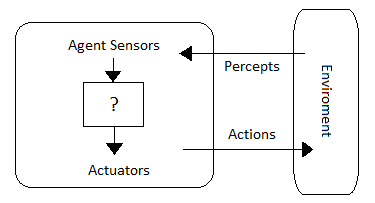
\includegraphics[width=\linewidth, height=3cm, keepaspectratio]{Pictures/ai-ml/agent-env-skeleton.png}
    \caption*{Agents interact with environments through sensors and actuators \cite{aci-1}}
\end{figure}

\begin{enumerate}
    \item An \textbf{agent} is anything that can be viewed as perceiving its \textbf{environment} through \textbf{sensors} and acting upon that environment through \textbf{actuators}.

    \item notion of desirability is captured by a \textbf{performance measure} that evaluates any given sequence of environment states.

    \item As a general rule, it is better to design performance measures according to what one actually wants in the environment, rather than according to how one thinks the agent should behave. 

    \item \textbf{information gathering}: Doing actions in order to modify future percepts
\end{enumerate}


\subsection{Agent}

\begin{enumerate}
    \item Mathematically speaking, we say that an agent’s behavior is described by the \textbf{agent function}\indexlabel{agent function} that maps any given percept sequence to an action.\\
    This an external characterization of the agent.

    \item Internally, the agent function for an artificial agent will be implemented by an \textbf{agent program}\indexlabel{agent program}.

    \item[] The agent function is an abstract mathematical description; the agent program is a concrete implementation, running within some physical system.\\
    SEE: \fullref{Agent Function VS Agent Program}

    \item A \textbf{rational agent} is one that does the right thing-conceptually speaking, every entry in the table for the agent function is filled out correctly. \\
    For each possible percept sequence, a rational agent should select an action that is expected to maximize its performance measure, given the evidence provided by the percept sequence and whatever built-in knowledge the agent has.

    \item An \textbf{omniscient agent} knows the actual outcome of its actions and can act accordingly; but omniscience is impossible in reality. 

    \item Rationality maximizes expected performance, while perfection maximizes actual performance.

    \item To the extent that an agent relies on the prior knowledge of its designer rather than on its own percepts, we say that the agent lacks \textbf{autonomy}.\\
    A rational agent should be autonomous-it should learn what it can to compensate for partial or incorrect prior knowledge. 
\end{enumerate}


\subsection{Environment}

\begin{enumerate}
    \item The environment is the external system or world in which the agent operates. It provides inputs (percepts) to the agent and reacts to the agent's actions. \cite{chatgpt}

    \item The “geography” of the environment is known \textbf{"a priori"} 
\end{enumerate}


\subsection{Sensor (input device) \cite{chatgpt}}

\begin{enumerate}
    \item A sensor is a device that allows an agent to perceive its environment. 
    
    \item It collects information from the environment, such as a camera capturing images or a thermometer measuring temperature.
\end{enumerate}


\subsection{Actuator (output device) \cite{chatgpt}}

\begin{enumerate}
    \item An actuator is a mechanism or device that the agent uses to take physical actions in the environment. 
    
    \item For example, in robotics, motors and servos are actuators that move parts of the robot.
\end{enumerate}


\subsection{Percepts (input)}

\begin{enumerate}
    \item \textbf{percept} refers to the agent’s perceptual inputs at any given instant

    \item \textbf{percept sequence} is the complete history of everything the agent has ever perceived

\end{enumerate}


\subsection{Actions (output)}

\begin{enumerate}
    \item an agent’s choice of action at any given instant can depend on the entire percept sequence observed to date, but not on anything it hasn’t perceived
\end{enumerate}



\section{Task Environment}

\begin{enumerate}
    \item task environments are essentially the “problems” to which rational agents are the “solutions.”

    \item "task environment" means "environment of task" in literal sense, but it actually means "scenario of task" or "task ecosystem"
\end{enumerate}

\subsection{PEAS description of task environment}
\begin{enumerate}
    \item P - Performance
    \item E - Environment
    \item A - Actuators
    \item S - Sensors
\end{enumerate}

Example:
\begin{customTableWrapper}{1.2}
\begin{table}[H]
    \centering
    \begin{tabular}{|l p{10cm}|}
        \hline
        \textbf{Task Environment} & automated taxi \\
        \hline\hline
        
        \textbf{Agent} & Taxi driver \\
        \hline

        \textbf{Performance Measure} & Safe, fast, legal, comfortable trip, maximize profits \\

        \textbf{Environment} & Roads, other traffic, pedestrians, customers \\

        \textbf{Actuators} & Steering, accelerator, brake, signal, horn, display \\

        \textbf{Sensors} & Cameras, sonar, speedometer, GPS, odometer, accelerometer, engine sensors, keyboard \\
        \hline
    \end{tabular}
\end{table}
\end{customTableWrapper}

\subsection{Properties of Task Environments}

\subsubsection{Observability}
\begin{enumerate}
    \item \textbf{Fully observable environment}: agent’s sensors give it access to the complete state of the environment at each point in time\\
    A task environment is effectively fully observable if the sensors detect all aspects that are relevant to the choice of action; relevance, in turn, depends on the performance measure.\\
    Fully observable environments are convenient because the agent need not maintain any internal state to keep track of the world. 

    \item \textbf{Partially observable environment}: An environment might be partially observable because of noisy and inaccurate sensors or because parts of the state are simply missing from the sensor data.

    \item \textbf{un-observable environment}: If the agent has no sensors at all then the environment is un-observable.\\
    One might think that in such cases the agent’s plight is hopeless, but the agent’s goals may still be achievable, sometimes with certainty. 

\end{enumerate}


\subsubsection{Single Agent VS Multi-agent}
\begin{enumerate}
    \item \textbf{Single Agent}: Only one agent operates on the environment.\\
    \textbf{For example}: an agent solving a crossword puzzle by itself is clearly in a single-agent environment. 

    \item \textbf{Multi-agent}: Multiple agents operate on same environment.\\
    \textbf{communication} often emerges as a rational behavior in multi-agent environments

    \begin{enumerate}
        \item \textbf{Competitive multi-agent environment}: multiple agents compete against each other for their own benefits\\
        in some competitive environments, \textbf{randomized behavior} is rational because it avoids the pitfalls of predictability\\
        \textbf{Example}: chess

        \item \textbf{Cooperative multi-agent environment}: multiple agents cooperate with each other for mutual benefits\\
        \textbf{Example}: multiple self driving cars in same environment
    \end{enumerate}
\end{enumerate}


\subsubsection{Deterministic VS stochastic}
\begin{enumerate}
    \item if next state of the environment is completely determined by the current state and the action executed by the agent, otherwise stochastic.

    \item \textbf{Non-deterministic}: which actions are characterized by their possible outcomes, but no probabilities are attached to them\\
    Non-deterministic environment descriptions are usually associated with performance measures that require the agent to succeed for all possible outcomes of its actions.
\end{enumerate}


\subsubsection{Uncertainty}
\begin{enumerate}
    \item an agent need not worry about \textbf{uncertainty} in a fully observable, deterministic environment

    \item We say an environment is \textbf{uncertain} if it is not fully observable or not deterministic.
\end{enumerate}


\subsubsection{Episodic VS sequential}

\begin{enumerate}
    \item \textbf{Episodic}: In an episodic task environment, the agent’s experience is divided into atomic episodes.\\
    In each episode the agent receives a percept and then performs a single action.\\
    Next episode does not depend on the actions taken in previous episodes.\\
    Episodic environments are much simpler than sequential environments because the agent does not need to think ahead.

    \item \textbf{Sequential}: In sequential environments, on the other hand, the current decision could affect all future decisions.
\end{enumerate}


\subsubsection{Static VS dynamic}
\begin{enumerate}
    \item If the environment can change while an agent is deliberating, then we say the environment is \textbf{dynamic} for that agent; otherwise, it is \textbf{static}.

    \item Static environments are easy to deal with because the agent need not keep looking at the world while it is deciding on an action, nor need it worry about the passage of time.\\
    \textbf{Example}: Crossword puzzles are static.

    \item Dynamic environments, on the other hand, are continuously asking the agent what it wants to do; if it hasn’t decided yet, that counts as deciding to do nothing. \\
    \textbf{Example}: Taxi driving is clearly dynamic: the other cars and the taxi itself keep moving while the driving algorithm dithers about what to do next.

    \item If the environment itself does not change with the passage of time but the agent’s performance score does, then we say the environment is \textbf{semi-dynamic}. \\
    \textbf{Example}: Chess, when played with a clock, is semi-dynamic.
\end{enumerate}


\subsubsection{Discrete vs. continuous}
\begin{enumerate}
    \item The discrete/continuous distinction applies to the state of the environment, to the way \textbf{time} is handled, and to the percepts and actions of the agent.

\paragraph*{Examples:}

    \item the chess environment has a finite number of distinct states (excluding the clock).\\
    Chess also has a discrete set of percepts and actions. 
    
    \item Taxi driving is a continuous-state and continuous-time problem: the speed and location of the taxi and of the other vehicles sweep through a range of continuous values and do so smoothly over time.\\
    Taxi-driving actions are also continuous (steering angles, etc.).\\
    Input from digital cameras is discrete, strictly speaking, but is typically treated as representing continuously varying intensities and locations.
\end{enumerate}


\subsubsection{Known vs. unknown}
\begin{enumerate}
    \item this distinction refers not to the environment itself but to the agent’s (or designer’s) state of knowledge about the “laws of physics” of the environment.

    \item In a \textbf{known environment}, the outcomes (or outcome probabilities if the environment is stochastic) for all actions are given.\\
    not the same as fully observable environments: It is quite possible for a known environment to be partially observable - for example, in solitaire card games, I know the rules but am still unable to see the cards that have not yet been turned over.

    \item if the environment is \textbf{unknown}, the agent will have to learn how it works in order to make good decisions.\\
    not the same as partially observable environments: an unknown environment can be fully observable - in a new video game, the screen may show the entire game state but I still don’t know what the buttons do until I try them. 
\end{enumerate}


\subsubsection*{Note}
\begin{enumerate}
    \item the hardest case is partially observable, multi-agent, stochastic, sequential, dynamic, continuous,and unknown.\\
    Taxi driving is hard in all these senses, except that for the most part the driver’s environment is known.\\
    Driving a rented car in a new country with unfamiliar geography and traffic laws is a lot more exciting. 

    \item \textbf{environment class}\indexlabel{environment class}: collection of environments

    \item \textbf{environment generator}: that selects particular environments (with certain likelihoods) in which to run the agent
\end{enumerate}

Examples of task environments and their characteristics \cite{aci-1}:
\begin{customTableWrapper}{1.2}
\begin{longtable}{|l|llllll|}
    \customTableHeaderColor
    \hline
    \textbf{Task Environment} & \textbf{Observable} & \textbf{Agents} & \textbf{Deterministic} & \textbf{Episodic} & \textbf{Static} & \textbf{Discrete} \\ 
    \hline\hline
    \endfirsthead

    \hline\endhead
    \hline\endfoot
    \hline\endlastfoot

    Crossword puzzle & Fully &  Single &  Deterministic & Sequential & Static & Discrete \\
    Chess with a clock & Fully & Multi & Deterministic & Sequential & Semi & Discrete \\
    
    \hline
    
    Poker & Partially & Multi & Stochastic & Sequential & Static&  Discrete \\
    Backgammon & Fully& Multi& Stochastic& Sequential& Static& Discrete\\
    
    \hline
    
    Taxi driving & Partially& Multi&  Stochastic& Sequential& Dynamic& Continuous\\
    Medical diagnosis& Partially & Single & Stochastic& Sequential& Dynamic& Continuous\\
    
    \hline
    
    Image analysis & Fully& Single& Deterministic& Episodic& Semi& Continuous\\
    Part-picking robot & Partially& Single& Stochastic& Episodic& Dynamic& Continuous\\
    
    \hline
    
    Refinery controller& Partially& Single& Stochastic& Sequential& Dynamic& Continuous\\
    Interactive English tutor & Partially& Multi& Stochastic& Sequential& Dynamic& Discrete\\

\end{longtable}
\end{customTableWrapper}


\chapter{AI Agents \cite{aci-1}}

\begin{center}
    \texttt{agent = architecture + program}
\end{center}

\begin{enumerate}
    \item \textbf{architecture}: computing device with physical sensors and actuators\\
    In general, the architecture makes the percepts from the sensors available to the program, runs the program, and feeds the program’s action choices to the actuators as they are generated.
    
    \item The job of AI is to design an \textbf{agent program} that implements the agent function - the mapping from percepts to actions.\\
    the program we choose has to be one that is appropriate for the architecture.\\
    If the program is going to recommend actions like Walk, the architecture had better have legs. 
\end{enumerate}

\section{Agent State Representation \cite{aci-1}}

\begin{figure}[H]
    \centering
    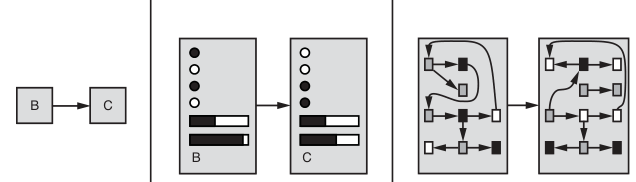
\includegraphics[width=\linewidth, height=2.5cm, keepaspectratio]{Pictures/ai-ml/agent-state-repr.png}
    \caption*{atomic, factored, and structured states}
\end{figure}

\begin{enumerate}
    \item \textbf{Atomic}
    \begin{enumerate}
        \item each state of the world is indivisible—it has no internal structure. 
    
        \item The algorithms underlying search and game-playing, Hidden Markov models, and Markov decision processes all work with atomic representations—or, at least, they treat representations as if they were atomic.

        \item if two different atomic states have nothing in common—they are just different black boxes
    \end{enumerate}

    \item \textbf{Factored}
    \begin{enumerate}
        \item A factored representation splits up each state into a fixed set of \textbf{variables} or \textbf{attributes}, each of which can have a \textbf{value}.

        \item two different factored states can share some attributes and not others; this makes it much easier to work out how to turn one state into another.

        \item With factored representations, we can also represent uncertainty\\
        \textbf{for example}, ignorance about the amount of gas in the tank can be represented by leaving that attribute blank.

        \item  Many important areas of AI are based on factored representations, including constraint satisfaction algorithms, propositional logic, planning, Bayesian networks, and the machine learning algorithms.
    \end{enumerate}

    \item \textbf{structured}
    \begin{enumerate}
        \item we need to understand the world as having things in it that are
related to each other, not just variables with values.

        \item Structured representations underlie relational databases and first-order logic, first-order probability models, knowledge-based learning and much of natural language understanding. 
        
        \item almost everything that humans express in natural language concerns objects and their relationships.
    \end{enumerate}

    \item  the axis along which atomic, factored, and structured representations lie is the axis of increasing \textbf{expressiveness}.\\
    a more expressive representation can capture, at least as concisely, everything a less expressive one can capture, plus some more.\\
    Often, the more expressive language is much more concise; for example, the rules of chess can be written in a page or two of a structured-representation language such as first-order logic but require thousands of pages when written in a factored-representation language such as propositional logic.\\
    On the other hand, reasoning and learning become more complex as the expressive power of the representation increases.\\
    To gain the benefits of expressive representations while avoiding their drawbacks, intelligent systems for the real world may need to operate at all points along the axis simultaneously.
\end{enumerate}

\section{Agent programs \cite{aci-1}}

\begin{enumerate}
    \item skeleton: they take the current percept as input from the sensors and return an action to the actuators. 
    
    \item agent program takes the current percept as input\\
    he agent program takes just the current percept as input because nothing more is available from the environment; if the agent’s actions need to depend on the entire percept sequence, the agent will have to remember the percepts.

    \item agent function takes the entire percept history
\end{enumerate}

\subsection{Table Driven Agent \cite{aci-1}}

\begin{algorithm}[H]
    \caption{The TABLE-DRIVEN-AGENT program is invoked for each new percept and returns an action each time. It retains the complete percept sequence in memory. \cite{aci-1}}

    \SetKwFunction{FUNCTION}{TABLE-DRIVEN-AGENT}
    \SetKwProg{Fn}{function}{:}{}
    \Fn{\FUNCTION{percept}}{
        \textbf{persistent}:\\
        \hspace{0.4cm} \textit{percepts}, a sequence, initially empty\\
        \hspace{0.4cm} \textit{table}, a table of actions, indexed by percept sequences, initially fully specified \\
        append \textit{percept} to the end of \textit{percepts} \\
        \textit{action} $\gets$ LOOKUP(\textit{percepts},\textit{table}) \\
        \Return \textit{action}
    }
\end{algorithm}

\vspace{0.3cm}

\begin{enumerate}
    \item If $\mathcal{P}$ be the set of possible percepts and let $\mathcal{T}$ be the lifetime of the agent (the total number of percepts it will receive), then The lookup table will contain $\dsum^T_{t=1} |P| ^t$ entries.

    \item Challenges if there are too many table entries:
    \begin{enumerate}
        \item storage space
        \item designer need time to create the table
        \item agent might never learn all the right table entries from its experience
        \item even if the environment is simple enough to yield a feasible table size, the designer still has no guidance about how to fill in the table entries
    \end{enumerate}

\end{enumerate}

\subsection{Simple reflex agents \cite{aci-1}}

\begin{table}[H]
    \begin{minipage}{0.4\linewidth}
        \begin{figure}[H]
            \centering
            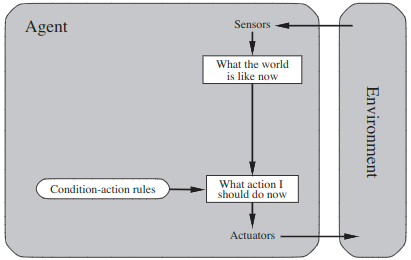
\includegraphics[width=\linewidth, height=4cm, keepaspectratio]{Pictures/ai-ml/agent--simple-reflex.png}
            \caption{Schematic diagram of a simple reflex agent}
        \end{figure}
    \end{minipage}
    \hfill
    \begin{minipage}{0.58\linewidth}
        \begin{algorithm}[H]
            \caption{simple reflex agent \cite{aci-1}}

            \SetKwFunction{FUNCTION}{SIMPLE-REFLEX-AGENT}
            \SetKwProg{Fn}{function}{:}{}
            \Fn{\FUNCTION{percept}}{
                \textbf{persistent}: \textit{rules}, a set of condition–action rules\\

                \textit{state} $\gets$ INTERPRET-INPUT(\textit{percept}) \\
                
                \textit{rule} $\gets$ RULE-MATCH(\textit{state,rules}) \\
                
                \textit{action} $\gets$ \textit{rule}.ACTION \\
                
                \textbf{return} \textit{action}
            }
        \end{algorithm}
    \end{minipage}
\end{table}

\vspace{0.3cm}

\begin{enumerate}
    \item The simplest kind of agent is the simple reflex agent. 
    
    \item These agents select actions on the basis of the current percept, ignoring the rest of the percept history.

    \item uses \textbf{condition–action rules} to map percepts to actions

    \item The \textbf{INTERPRET-INPUT function} generates an abstracted description of the current state from the percept, and the \textbf{RULE-MATCH function} returns the first rule in the set of rules that matches the given state description.

    \item Note that the description in terms of “rules” and “matching” is purely conceptual; actual implementations can be as simple as a collection of logic gates implementing a Boolean circuit.

\subsubsection*{DISADVANTAGES:}

    \item limited intelligence
    
    \item environment needs to be fully observable. Even a little bit of unobservability can cause serious trouble.
    
    \item Infinite loops are often unavoidable for simple reflex agents operating in partially observable environments\\
    \textbf{Solution}: Escape from infinite loops is possible if the agent can randomize its actions.\\
    In single-agent environments, randomization is usually not rational.\\
    It is a useful trick that helps a simple reflex agent in some situations, but in most cases we can do much better with more sophisticated deterministic agents. 
\end{enumerate}



\subsection{Model-based reflex agents \cite{aci-1}}

\begin{table}[H]
    \begin{minipage}{0.4\linewidth}
        \begin{figure}[H]
            \centering
            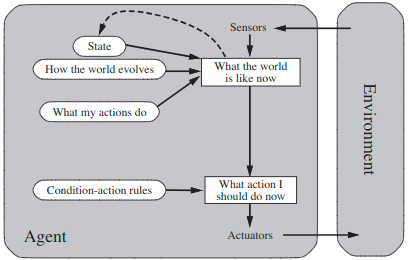
\includegraphics[width=\linewidth, height=4cm, keepaspectratio]{Pictures/ai-ml/agent--model-based-reflex.png}
            \caption{Model-based reflex agent}
        \end{figure}
    \end{minipage}
    \hfill
    \begin{minipage}{0.58\linewidth}
        \begin{algorithm}[H]
            \caption{model-based reflex agent \cite{aci-1}}

            \SetKwFunction{FUNCTION}{MODEL-BASED-REFLEX-AGENT}
            \SetKwProg{Fn}{function}{:}{}
            \Fn{\FUNCTION{percept}}{
                \textbf{persistent}:\\
                
                \hspace{0.4cm} \textit{state}, the agent’s current conception of the world state \\
                \hspace{0.4cm} \textit{model}, a description of how the next state depends on current state and action \\
                \hspace{0.4cm} \textit{rules}, a set of condition–action rules \\
                \hspace{0.4cm} \textit{action}, the most recent action, initially none \\

                \textit{state} $\gets$ UPDATE-STATE(\textit{state, action, percept, model}) \\
                
                \textit{rule} $\gets$ RULE-MATCH(\textit{state, rules}) \\
                
                \textit{action} $\gets$ \textit{rule}.ACTION \\
                
                \textbf{return} \textit{action}
            }
        \end{algorithm}
    \end{minipage}
\end{table}

\vspace{0.3cm}


\begin{enumerate}
    \item keeps track of the part of the world it can’t see now. (handle partial observability)\\
    The agent maintains some sort of \textbf{internal state} that depends on the percept history and thereby reflects at least some of the unobserved aspects of the current state.

    \item Updating this internal state information as time goes by requires two kinds of knowledge to be encoded in the agent program.
    \begin{enumerate}
        \item we need some information about how the world evolves independently of the agent

        \item we need some information about how the agent’s own actions affect the world
    \end{enumerate}
    This knowledge about “\textit{how the world works}” is called a \textbf{model} of the world. 

    \item The details of how models and states are represented vary widely depending on the type of environment and the particular technology used in the agent design. 

    \item Regardless of the kind of representation used, it is seldom possible for the agent to determine the current state of a partially observable environment exactly.\\
    Instead, the box\ mechanism labeled “what the world is like now” represents the agent’s “best guess” (or sometimes best guesses).
\end{enumerate}


\subsection{(Model-based) Goal-based agents \cite{aci-1}}

\begin{enumerate}
    \item as well as a current state description, the agent needs some sort of \textbf{goal} information that describes situations that are desirable

    \item \textbf{Search} and \textbf{planning} are the subfields of AI devoted to finding action sequences that achieve the agent’s goals.

    \item Although the goal-based agent appears less efficient, it is more flexible because the knowledge that supports its decisions is represented explicitly and can be modified.\\
    If it starts to rain, the agent can update its knowledge of how effectively its brakes will operate; this will automatically cause all of the relevant behaviors to be altered to suit the new conditions.\\
    For the reflex agent, on the other hand, we would have to rewrite many condition–action rules. 

    \item Goals alone are not enough to generate high-quality behavior in most environments.
\end{enumerate}


\begin{table}[h]
    \begin{minipage}{0.49\linewidth}
        \begin{figure}[H]
            \centering
            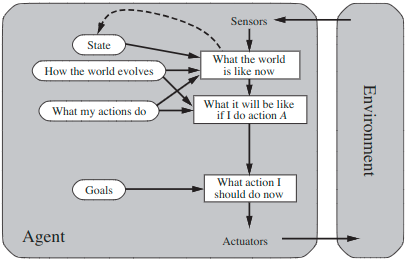
\includegraphics[width=\linewidth, height=4cm, keepaspectratio]{Pictures/ai-ml/agent--model-based-goal-based.png}
            \caption{Model-based goal-based agent \cite{aci-1}}
        \end{figure}
    \end{minipage}
    \hfill
    \begin{minipage}{0.49\linewidth}
        \begin{figure}[H]
            \centering
            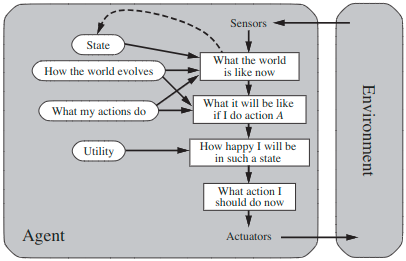
\includegraphics[width=\linewidth, height=4cm, keepaspectratio]{Pictures/ai-ml/agent--model-based-utility-based.png}
            \caption{Model-based utility-based agent \cite{aci-1}}
        \end{figure}
    \end{minipage}
\end{table}

\subsection{Utility-based agents \cite{aci-1}}

\begin{enumerate}
    \item Many action sequences can lead to same goal, but some sequences are more favourable than others.\\
    Goals just provide a crude binary distinction between “happy” and “unhappy” states.\\
    A more general performance measure should allow a comparison of different world states according to exactly how happy they would make the agent.\\
    Because “happy” does not sound very scientific, economists and computer scientists use the term \textbf{utility} instead.

    \item An agent’s \textbf{utility function} is essentially an internalization of the performance measure. 
    
    \item If the internal utility function and the external performance measure are in agreement, then an agent that chooses actions to maximize its utility will be rational according to the external performance measure. 

    \item like goal-based agents, a utility-based agent has many advantages in terms of flexibility and learning.

    \item in two kinds of cases, goals are inadequate but a utility-based agent can still make rational decisions. 
    \begin{enumerate}
        \item when there are conflicting goals, only some of which can be achieved (for example, speed and safety), the utility function specifies the appropriate tradeoff.

        \item when there are several goals that the agent can aim for, none of which can be achieved with certainty, utility provides a way in which the likelihood of success can be weighed against the importance of the goals. 
    \end{enumerate}

    \item An agent that possesses an \textbf{\textit{explicit} utility function} can make rational decisions with a general-purpose algorithm that does not depend on the specific utility function being maximized.\\
    In this way, the “global” definition of rationality—designating as rational those agent functions that have the highest performance—is turned into a “local” constraint on rational-agent designs that can be expressed in a simple program.

    \item A utility-based agent has to model and keep track of its environment, tasks that have involved a great deal of research on perception, representation, reasoning, and learning. \\
    Choosing the utility-maximizing course of action is also a difficult task, requiring ingenious algorithms.
\end{enumerate}


\subsection{Learning Agent \cite{aci-1}}

\begin{figure}[H]
    \centering
    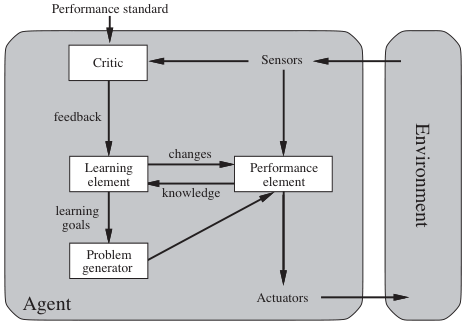
\includegraphics[width=\linewidth, height=4cm, keepaspectratio]{Pictures/ai-ml/agent--learning.png}
    \caption{General Learning Agent \cite{aci-1}}
\end{figure}


\begin{enumerate}
    \item Learning allows the agent to operate in initially unknown environments and to become more competent than its initial knowledge alone might allow.

    \item A learning agent can be divided into four conceptual components:
    \begin{enumerate}
        \item \textbf{learning element}: responsible for making improvements

        \item \textbf{performance element}: responsible for selecting external actions\\
        it takes in percepts and decides on actions

        \item \textbf{critic}: provides feedback on how the agent is doing and determines how the performance element should be modified to do better in the future\\
        The critic tells the learning element how well the agent is doing with respect to a fixed performance standard.\\
        The critic is necessary because the percepts themselves provide no indication of the agent’s success.

        \item \textbf{problem generator}: It is responsible for suggesting actions that will lead to new and informative experiences.\\
        The point is that if the performance element had its way, it would keep doing the actions that are best, given what it knows.\\
        But if the agent is willing to explore a little and do some perhaps sub-optimal actions in the short run, it might discover much better actions for the long run.\\
        The problem generator’s job is to suggest these exploratory actions.
    \end{enumerate}

    \item  the \textbf{performance standard} distinguishes part of the
incoming percept as a reward (or penalty) that provides direct feedback on the quality of the
agent’s behavior.    
\end{enumerate}



\subsection{problem-solving agent \cite{aci-1}}

\begin{enumerate}
    \item Problem-solving agents use \textbf{atomic} representations, states of the world are considered as wholes, with no internal structure visible to the problem-solving algorithms. 

    \item \textbf{uninformed search algorithms}—algorithms that are given no information about the problem other than its definition.

    \item \textbf{Informed search algorithms} can do quite well given some guidance on where to look for solutions

    \item \textbf{Goals} help organize behavior by limiting the objectives that the agent is trying to achieve and hence the actions it needs to consider.\\
    \textbf{Goal formulation}, based on the current situation and the agent’s performance measure, is the first step in problem solving.\\
    We consider a goal to be a set of world states—exactly those states in which the goal is satisfied.\\
    The agent’s task is to find out how to act, now and in the future, so that it reaches a goal state.

    \item  \textbf{Problem formulation} is the process of deciding what actions and states to consider, given a goal. 

    \item The process of looking for a sequence of actions that reaches the goal is called \textbf{search}.

    \item A search algorithm takes a problem as input and returns a \textbf{solution} in the form of an \textbf{action sequence}.\\
    Solution quality is measured by the path cost function, and an \textbf{optimal solution} has the lowest path cost among all solutions.

    \item Once a solution is found, the actions it recommends can be carried out. This is called the \textbf{execution phase}.

    \item A \textbf{problem} can be defined formally by five components:
    \begin{enumerate}
        \item The \textbf{initial state} that the agent starts in.

        \item A description of the possible \textbf{actions} available to the agent.\\
        Given a particular state \textit{s}, \verb|ACTIONS(s)| returns the set of actions that can be executed in \textit{s}.\\
        We say that each of these actions is \textbf{applicable} in \textit{s}.

        \item A description of what each action does; the formal name for this is the \textbf{transition model}, specified by a function \verb|RESULT(s, a)| that returns the state that results from doing action \textit{a} in state \textit{s}.\\
        We also use the term \textbf{successor} to refer to any state reachable from a given state by a single action.\\
        Together, the initial state, actions, and transition model implicitly define the \textbf{state space} of the problem—the set of all states reachable from the initial state by any sequence of actions.\\
        The state space forms a directed network or graph in which the nodes are states and the links between nodes are actions.\\
         A \textbf{path} in the state space is a sequence of states connected by a sequence of actions.

        \item \textbf{goal test} determines whether a given state is a goal state.

        \item The \textbf{step cost} of taking action $a$ in state $s$ to reach state $s'$ is denoted by $c(s, a, s')$.\\
        A \textbf{path cost} function that assigns a numeric cost to each path.\\
        The problem-solving agent chooses a cost function that reflects its own performance measure.\\
        we assume that the cost of a path can be described as the \textbf{sum} of the costs of the individual actions along the path.
    \end{enumerate}

    \item A \textbf{toy problem}\indexlabel{toy problem} is intended to illustrate or exercise various problem-solving methods.\\
    It can be given a concise, exact description and hence is usable by different researchers to compare the performance of algorithms.

    \item A \textbf{real-world problem}\indexlabel{real-world problem} is one whose solutions people actually care about.\\
    Such problems tend not to have a single agreed-upon description, but we can give the general flavor of their formulations.
\end{enumerate}

\begin{figure}[H]
    \centering
    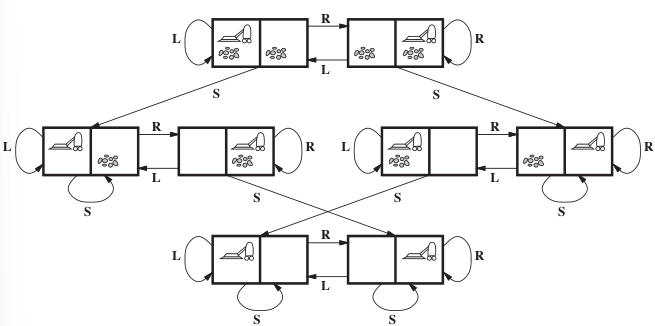
\includegraphics[width=\linewidth, height=6cm, keepaspectratio]{Pictures/ai-ml/vaccum-toy-states.png}
    \caption*{The state space for the vacuum world. Links denote actions: L = Left, R = Right, S = Suck.}
\end{figure}

\begin{customTableWrapper}{1.3}
\begin{longtable}{|p{3cm} p{10cm}|}
    \hline\endfirsthead
    \hline\endhead
    \hline\endfoot
    \hline\endlastfoot

    \textbf{States} & The state is determined by both the agent location and the dirt locations. \\ 
    \hline

    \textbf{Initial state} & Any state can be designated as the initial state.\\
    \hline

    \textbf{Actions} & In this simple environment, each state has just three actions: Left, Right, and Suck.\\
    \hline

    \textbf{Transition model} & The actions have their expected effects, except that moving Left in the leftmost square, moving Right in the rightmost square, and Sucking in a clean square have no effect. \\
    \hline

    \textbf{Goal test} & This checks whether all the squares are clean.\\
    \hline

    \textbf{Path cost} & Each step costs 1, so the path cost is the number of steps in the path.\\
    \hline
\end{longtable}
\end{customTableWrapper}

\begin{algorithm}[h]
    \caption*{A simple problem-solving agent. It first formulates a goal and a problem, searches for a sequence of actions that would solve the problem, and then executes the actions one at a time. When this is complete, it formulates another goal and starts over. \cite{aci-1}}

    \SetKwFunction{FUNCTION}{SIMPLE-PROBLEM-SOLVING-AGENT}
    \SetKwProg{Fn}{function}{:}{}
    \Fn{\FUNCTION{percept}}{
        \textbf{persistent}:\\
        \hspace{0.4cm} \textit{seq}, an action sequence, initially empty \\
        \hspace{0.4cm} \textit{state}, some description of the current world state \\
        \hspace{0.4cm} \textit{goal}, a goal, initially null \\
        \hspace{0.4cm} \textit{problem}, a problem formulation\\
        
        state $\gets$ UPDATE-STATE(\textit{state, percept})\\
        \If{\textit{seq} is empty}{
            \textit{goal} $\gets$ FORMULATE-GOAL(\textit{state})\\
            
            \textit{problem} $\gets$ FORMULATE-PROBLEM(\textit{state, goal})\\
            
            \textit{seq} $\gets$ SEARCH(\textit{problem})\\
            
            \If{\textit{seq} = \textit{failure}}{
                \textbf{return} a null action
            }
        }
        \textit{action} $\gets$ FIRST(\textit{seq})\\
        \textit{seq} $\gets$ REST(\textit{seq})\\
        \textbf{return} \textit{action}
    }
\end{algorithm}


\subsubsection{Measuring problem-solving performance \cite{aci-1}}

\begin{customTableWrapper}{1.2}
\begin{table}[H]
    \centering
    \begin{tabular}{l p{10cm}}
        \textbf{Completeness} & Is the algorithm guaranteed to find a solution when there is one? \\
        
        \textbf{Optimality} & Does the strategy find the optimal solution? \\
        
        \textbf{Time complexity} & How long does it take to find a solution? \\
        
        \textbf{Space complexity} & How much memory is needed to perform the search?\\
    \end{tabular}
\end{table}
\end{customTableWrapper}


\begin{customTableWrapper}{1.2}
\begin{table}[H]
    \centering
    \begin{tabular}{l p{10cm}}
        $V$ & set of vertices (nodes) of the graph \\
        
        $E$ & set of edges (links) \\

        $b$ & \textbf{branching factor} or maximum number of successors of any node\\

        $d$ & \textbf{depth} of the shallowest goal node (i.e., the number of steps along the path from the root)\\

        $m$ &  maximum length of any path in the state space\\
    \end{tabular}
    \caption*{Notation}
\end{table}
\end{customTableWrapper}



\begin{enumerate}
    \item Time and space complexity are always considered with respect to some measure of the problem difficulty. 
    
    \item In theoretical computer science, the typical measure is the size of the state space graph, $|V| + |E|$.

    \item \textbf{search cost}: typically depends on the time complexity but can also include a term for memory usage

    \item \textbf{total cost}: combines the search cost and the path cost of the solution found
\end{enumerate}





\subsection{planning agents \cite{aci-1}}

\begin{enumerate}
    \item Goal-based agents that use more advanced \textbf{factored} or \textbf{structured} representations are usually called \textbf{planning agents}.


\end{enumerate}





% 79/1153


































































\chapter{AI Agent Solution Searching \cite{aci-1}}

\begin{enumerate}
    \item A \textbf{solution} is an action sequence, so search algorithms work by considering various possible action sequences. 
    
    \item The possible action sequences starting at the initial state form a \textbf{search tree} with:
    \begin{enumerate}
        \item the initial state at the root
        \item the branches are actions
        \item the nodes correspond to states in the state space of the problem
    \end{enumerate}

    \item \textbf{expanding} the current state: applying each legal action to the current state, thereby \textbf{generating} a new set of states

    \item  essence of search—following up one option now and putting the others aside for later, in case the first choice does not lead to a solution.

    \item \textbf{leaf node}: a node with no children in the tree.

    \item \textbf{frontier}/ \textbf{open list}: The set of all leaf nodes available for expansion at any given point\\
    the frontier separates the state-space graph into the explored region and the unexplored region, so that every path from the initial state to an unexplored state has to pass through a state in the frontier

    \item \textbf{explored set} / \textbf{closed list}: remembers every expanded node

    \item The process of expanding nodes on the frontier continues until either a solution is found or there are no more states to expand.

    \item \textbf{search strategy}: how they choose which state to expand next
\end{enumerate}


SEE:
\begin{enumerate}
    \item \fullref{Tree Search (generic)}
    \item \fullref{Graph Search (generic)}
    
    \item Uninformed:
    \begin{enumerate}
        \item \fullref{Breadth-first search BFS}
        \item \fullref{Uniform-cost search (UCS)}
        \item \fullref{Depth-first search (DFS)}
        \item \fullref{Depth-limited search (DLS)}
        \item \fullref{Iterative deepening depth-first search/ Iterative deepening search (IDS)}
        \item \fullref{Iterative Lengthening Search (ILS)}
        \item \fullref{Bidirectional search}
    \end{enumerate}
    
    \item Informed:
    \begin{enumerate}
        \item 
    \end{enumerate}
\end{enumerate}


\section{Node of a tree/ graph (n)}
\begin{table}[H]
    \centering
    \begin{tabular}{l p{8cm}}
        \textit{n}.STATE & the state in the state space to which the node corresponds \\
        
        \textit{n}.PARENT & the node in the search tree that generated this node\\
        
        \textit{n}.ACTION &  the action that was applied to the parent to generate the node \\
        
        \textit{n}.PATH-COST & the cost, traditionally denoted by $g(n)$, of the path from the initial state to the node, as indicated by the parent pointers.
    \end{tabular}
\end{table}


\begin{algorithm}
    \caption{ function CHILD-NODE takes a parent node and an action and returns the resulting child node}

    \SetKwFunction{FUNCTION}{CHILD-NODE}
    \SetKwProg{Fn}{function}{:}{}
    \Fn{\FUNCTION{problem, parent, action}}{
        \Return a node with \\
        \hspace{0.4cm} STATE = \textit{problem}.RESULT(\textit{parent}.STATE, \textit{action}), \\
        \hspace{0.4cm} PARENT = \textit{parent},  \\
        \hspace{0.4cm} ACTION = \textit{action},\\
        \hspace{0.4cm} PATH-COST = \textit{parent}.PATH-COST + \textit{problem}.STEP-COST(\textit{parent}.STATE, \textit{action})
    }
\end{algorithm}

































































